\documentclass[twoside]{article}

\usepackage{aistats2019}
% If your paper is accepted, change the options for the package
% aistats2019 as follows:
%
%\usepackage[accepted]{aistats2019}
%
% This option will print headings for the title of your paper and
% headings for the authors names, plus a copyright note at the end of
% the first column of the first page.

% If you set papersize explicitly, activate the following three lines:
%\special{papersize = 8.5in, 11in}
%\setlength{\pdfpageheight}{11in}
%\setlength{\pdfpagewidth}{8.5in}

% If you use natbib package, activate the following three lines:
%\usepackage[round]{natbib}
%\renewcommand{\bibname}{References}
%\renewcommand{\bibsection}{\subsubsection*{\bibname}}

% If you use BibTeX in apalike style, activate the following line:
%\bibliographystyle{apalike}


\usepackage{fullpage,amsthm}

\usepackage{graphicx} % support the \includegraphics command and options
\usepackage{array} % for better arrays (eg matrices) in maths
%\usepackage{paralist} % very flexible & customisable lists (eg. enumerate/itemize, etc.)
\usepackage{amsmath, amssymb, color, verbatim}
\usepackage{hyphenat,epsfig,subfigure,multirow}
\usepackage{hyperref}

\usepackage{algorithm,algorithmic}


\usepackage{algorithm,algorithmic}


\newtheorem{theorem}{Theorem}[section]
\newtheorem{lemma}[theorem]{Lemma}
\newtheorem{proposition}[theorem]{Proposition}
\newtheorem{corollary}[theorem]{Corollary}
\newtheorem{claim}[theorem]{Claim}
\newtheorem{fact}[theorem]{Fact}
\newtheorem{conj}[theorem]{Conjecture}
\newtheorem{definition}{Definition}[section]
%\theoremstyle{definition}
\newtheorem{remark}[theorem]{Remark}

\newenvironment{proofof}[1]{\begin{proof}[of {#1}]}{\end{proof}}

\newcommand{\mypar}[1]{\smallskip \noindent {\bf {#1}.}}
\newcommand{\myparq}[1]{\smallskip \noindent {\bf {#1}}}

\DeclareMathOperator*{\argmax}{arg\,max}
%\newenvironment{proof}[1][Proof]{\begin{trivlist}
%\item[\hskip \labelsep {\bfseries #1}]}{\end{trivlist}}
%\newenvironment{definition}[1][Definition]{\begin{trivlist}
%\item[\hskip \labelsep {\bfseries #1}]}{\end{trivlist}}
\newenvironment{example}[1][Example]{\begin{trivlist}
		\item[\hskip \labelsep {\bfseries #1}]}{\end{trivlist}}
% \newenvironment{remark}[1][Remark]{\begin{trivlist}
% \item[\hskip \labelsep {\bfseries #1}]}{\end{trivlist}}

\renewcommand{\qed}{\nobreak \ifvmode \relax \else
	\ifdim\lastskip<1.5em \hskip-\lastskip
	\hskip1.5em plus0em minus0.5em \fi \nobreak
	\vrule height0.75em width0.5em depth0.25em\fi}

\newcommand{\ie}{{\it i.e.,\ }}
\newcommand{\eg}{{\it e.g.,\ }}
\newcommand{\etal}{{\it et al.\,}}
\newcommand{\through}{,\ldots,}
\newcommand{\cala}{\mathcal A}
\newcommand{\calb}{\mathcal B}
\newcommand{\calgn}{{\mathcal G}_n}
%\newcommand{\HHH}{\mathcal H}
%\newcommand{\DDD}{\mathcal D}
%\newcommand{\XXX}{\mathcal X}
\newcommand{\cals}{\mathcal S}
%\newcommand{\RRR}{\mathcal R}
\newcommand{\eps}{\epsilon}
\newcommand{\z}{\mathrm{z}}
\newcommand{\zo}{\{0,1\}}
\newcommand{\oo}{\{+1,-1\}}
\newcommand{\inv}{^{-1}}
\def\E{\mathop{\mathbb{E}}\displaylimits}
\def\poly{\mathop{\rm{poly}}\nolimits}
\def\Lap{\mathop{\rm{Lap}}\nolimits}
\newcommand{\Cauchy}{\operatorname{Cauchy}}
\newcommand{\inr}{\in_{\mbox{\tiny R}}}
\newcommand{\cP}{\mathcal P}




\begin{document}

% If your paper is accepted and the title of your paper is very long,
% the style will print as headings an error message. Use the following
% command to supply a shorter title of your paper so that it can be
% used as headings.
%
%\runningtitle{I use this title instead because the last one was very long}

% If your paper is accepted and the number of authors is large, the
% style will print as headings an error message. Use the following
% command to supply a shorter version of the authors names so that
% they can be used as headings (for example, use only the surnames)
%
%\runningauthor{Surname 1, Surname 2, Surname 3, ...., Surname n}

\twocolumn[

\aistatstitle{Hierarchical Clustering for Euclidean Data}

\aistatsauthor{Moses Charikar \And Vaggos Chatziafratis \And  Rad Niazadeh \And Grigory Yaroslavtsev }

\aistatsaddress{Stanford University \And  Stanford University \And Stanford University \And Indiana  University, Bloomington } ]

\begin{abstract}
  The Abstract paragraph should be indented 0.25 inch (1.5 picas) on
  both left and right-hand margins. Use 10~point type, with a vertical
  spacing of 11~points. The \textbf{Abstract} heading must be centered,
  bold, and in point size 12. Two line spaces precede the
  Abstract. The Abstract must be limited to one paragraph.
\end{abstract}

\section{Introduction}

The goal of this project is to extend Dasgupta's hierarchical clustering paradigm to Euclidean datasets.
Recall that in the graphical case given a graph $G(V,E)$ and a tree $\mathcal T$ whose nodes correspond to vertices in the graph Dasgupta's hierarchical clustering cost is defined as follows:
$$f^-(\mathcal T) = \sum_{(i,j) \in E} w_{ij} |\{x \in T(i,j)\}|,$$
where $T(i,j)$ is the subtree of $\mathcal T$ rooted in the least common ancestor of $i$ and $j$ in $\mathcal T$.
Here $w(i,j)$ corresponds to a given similarity measure between vertices $i$ and $j$.
For the general case the best known approximation is $O(\sqrt{\log |V|})$ using the sparsest cut algorithm. Furthermore, under SSE-conjecture no algorithm can get a constant factor approximation in polynomial time~\cite{CC17}

We also consider a complementary objective which one aims to maximize:
$$f^+(\mathcal T) = \sum_{(i,j) \in E} w_{ij} (|V| - |\{x \in T(i,j)\}|),$$


Consider a set of vectors $v_1, \dots, v_n \in \mathbb R^d$. In this case the similarity measure $w$ only depends on the underlying vectors, i.e. $w_{ij} = f(v_i, v_j)$ for some function $f \colon \mathbb R \times \mathbb R \to [0,1]$.
\begin{definition}[Monotone distance-based similarity measure]
	A similarity measure $w_{ij} = f(v_i, v_j)$ is \emph{distance-based} if $f(v_i, v_j) = g(\|v_i - v_j\|_2)$ for some function $g \colon \mathbb R \to [0,1]$.
	A similarity measure $w_{ij}$ is \emph{monotone distance-based} if furthermore $g \colon \mathbb R \to [0,1]$ is a monotone non-increasing function.
\end{definition}

As a specific example of a monotone distance-based similarity measure it is natural to consider the Gaussian kernel similarity, i.e.: 
$$w_{ij} = (\sqrt{2 \pi} \sigma)^{-n} e^{- \frac{\|v_i - v_j\|_2^2}{2\sigma^2}},$$ 
where $\sigma$ is a normalization factor. Below we will ignore the multiplicative factor as it doesn't affect multiplicative approximations. We will also set $\sigma = 1/\sqrt{2}$ to simplify the presentation.

\textbf{Question:} Is it possible to get a better approximation and/or faster algorithm for the Hierarchical clustering problem in this setting? Or can hard instances of the general case be embedded into a into vectors with weights from the Gaussian kernel?

\section{Tight cases for Average-Linkage for $f^+$}

\subsection{High-dimensional case}
For $i \in [n^{2/3}]$ and $j \in [n^{1/3}]$ let $v_{i,j} = \Delta (e_i + (1 + \epsilon)e_{k + j})$ where $k = n^{2/3}$.
Then it is easy to see that for any fixed $i \in [n^{2/3}]$ and $j_1 \neq j_2 \in [n^{1/3}]$ it holds that:
$$\|v_{i,j_1} - v_{i, j_2}\|_2^2 = 2 (1 + \epsilon)^2 \Delta^2$$
For any fixed $j \in [n^{1/3}]$ and $i_1 \neq i_2 \in [n^{2/3}]$ it holds that:
$$\|v_{i_1, j} - v_{i_2,j}\|_2^2 = 2 \Delta^2.$$
Otherwise if $i_1 \neq i_2 \in [n^{2/3}]$ and $j_1 \neq j_2  \in [n^{1/3}]$ then:
$$\|v_{i_1, j_1} - v_{i_2, j_2}\|_2^2 = 2 \Delta^2 + 2 (1 + \epsilon)^2 \Delta^2 \ge 4 \Delta^2.$$

By setting $\Delta^2 > c \log n$ for a sufficiently large constant $c$ the contribution of pairs of vectors with $i_1 \neq i_2$ and $j_1 \neq j_2$ can be made negligible. 
The rest of the pairs correspond to an embedded hard instance from Charikar, Chatziafratis and Niazadeh (SODA'19 submission) for which average-linkage only achieves a $\frac13$-approximation compared to the optimum.

Using JL-transform we can reduce the dimension required for the above reduction to $d = O(\log n)$.

\subsection{Low-dimensional case}

For $d = 1$ the hardest instance seems to be the following.
Take four equally spaced points on a line, i.e. $0, \Delta, 2\Delta, 3 \Delta$.
Then the average-linkage clustering algorithm might first connect the two middle points and then connect the two other points in arbitrary order.
We denote the cost of this solution as $AVG$.
An alternative solution would be to create two groups $(0, \Delta)$ and $(2\Delta, 3\Delta)$ and then merge them together.
We denote the cost of this solution as $OPT$.
By making $\Delta$ sufficiently large the contribution of pairs at distance more than $\Delta$ from each other can be ignored. We thus have:
\begin{align*}
AVG \approx 3 e^{-\Delta^2} \\
OPT \approx 4 e^{- \Delta^2},
\end{align*}
which gives the ratio of $4/3$.

\textbf{Question:} Is the $4/3$ ratio achievable by average-linkage clustering for $d = 1$?


\section{Hierarchical Clustering in 1D}
We first consider the case $d = 1$.
In this case the input can be represented as points on a line, which we assume to be sorted without loss of generality, i.e. $x_1 \le \dots  \le x_n$.

\subsection{Average-Linkage}
\begin{theorem}\label{thm:average-linkage}
	For $d = 1$ under any monotone distance-based similarity measure $w_{ij} = g(x_i, x_j)$ the algorithm \textsc{Average Linkage} gives a $\frac12$-approximation for the objective $f^+$.
\end{theorem}

\begin{proof}
	For ease of notation from now on, for any two sets $A,B$, we denote $\sum_{i\in A,j\in B}w_{ij}$ by simply using $w_{AB}$.
	The proof is based on a potential function argument. We prove that at every step, \textsc{Average Linkage} gets at least $50\%$ of the total available potential.
	
	\begin{figure}[h!]
		\centering
		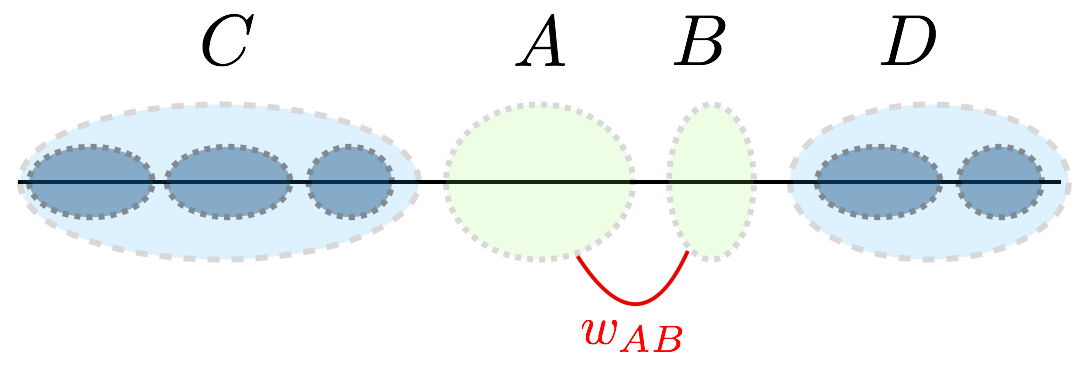
\includegraphics[width=9cm]{merging}
		\caption{Illustration of how the merging process looks like in the 1-dimensional case.}
	\end{figure}
	
	We focus on a single step of \textsc{Average Linkage}, where neighboring clusters $A,B$ just got merged. As we see in the figure, let $C$ denote the nodes on the left of $A$ and $D$ denote the nodes on the right of $B$. Observe that $C,D$ may be empty sets. The initial total available potential is:
	\[
	\Phi_0 = (n-2)\sum_{e\in E}w_e
	\]
	At a generic step of \textsc{Average Linkage}, by merging two clusters $A,B$, the difference in potential is:
	\[
	\Delta\Phi(A,B) = w_{AB}(|C|+|D|) + w_{AC}|B|+ w_{BD}|A| 
	\]
	
	By merging $A,B$, \textsc{Average Linkage} gains a contribution of:
	\[
	\textsc{Average Linkage}(A,B) = w_{AB}(|C|+|D|)
	\]
	
	However, after the merge, \textsc{Average Linkage} can no longer gain any contribution because of nodes in $B$ and edges between $A,C$ or because of nodes in $A$ and edges between $B,D$. More specifically, out of the total available potential at this step, $w_{AC}|B| + w_{BD}|A|$ is lost. We show that what \textsc{Average Linkage} gained at this step is no less than what \textsc{Average Linkage} lost, i.e.:
	\[
	w_{AB}(|C|+|D|) \ge w_{AC}|B| + w_{BD}|A|
	\]
	
	From the \textsc{Average Linkage} criterion:
	\[
	\dfrac{w_{AB}}{|A||B|}\ge \dfrac{w_{AC}}{|A||C|}\implies w_{AB}|C| \ge w_{AC}|B|
	\]
	\[
	\dfrac{w_{AB}}{|A||B|}\ge \dfrac{w_{BD}}{|B||D|}\implies w_{AB}|D| \ge w_{BD}|A|
	\]
	
	By summing up we get the desired inequality which means that:
	\[
	\textsc{Average Linkage}(A,B)\ge \dfrac12 \Delta\Phi(A,B)
	\]
	
	At the end of the merging process, the final potential $\Phi_{n-1} = 0$, so in total:
	\[
	\textsc{Average Linkage}\ge \dfrac12 (n-2)\sum_{e\in E}w_e\ge \dfrac12 OPT
	\]
	
\end{proof}

\section{Hierarchical Clustering in High Dimensions}
The input is $v_1, \dots v_n \in \mathbb R^d$. Consider an algorithm which picks a random Gaussian vector $g \sim N_d(0,1)$, projects on it and then partitions the resulting points by uniformly random cuts. Here by a uniformly random cut we mean the following process. Let $x_i = \langle v_i, g \rangle$ and assume $x_1 \le \dots \le x_n$. Pick $y \sim U([x_1, x_n])$ and split the set of points into $L = \{i \colon x_i \le y\}$ and $R = \{i \colon x_i > y\}$, then apply the same algorithm recursively on $L$ and $R$.

Fix any triangle $(v_i, v_j, v_k)$. Conditioned on cutting this triangle for the first time let $(p_{ij},p_{ik},p_{jk})$ be the vector of probabilities corresponding to the events that the corresponding edge is not cut. I.e. this is the probability that we score the contribution of this edge in the objective. Note that $p_{ij} + p_{ik} + p_{jk} = 1$.

Conisder any triangle whose vertices are $v_i, v_j, v_k$. To simplify presentation we set $i = 1, j = 2, k = 3$. We can assume that $\|v_2 - v_1\| \ge \|v_2 - v_3\| \ge \|v_1 - v_3\|$. Let $\theta_1 = \widehat{v_1 - v_3, v_2 - v_3}$, $\theta_2 = \widehat{v_2 - v_1, v_3 - v_1}$ and $\theta_3 = \widehat{v_1 - v_2, v_3 - v_2}$ so that $\theta_1 \ge \theta_2 \ge \theta_3$.

The probability that the $i$-the longest side of the triangle has the longest projection is then $\theta_i/\pi$. Conditioned on $(v_1, v_2)$ having the longest projection the probability of scoring the contribution of $(v_2, v_3)$ is given as:

$$\frac{1}{\theta_1} \int_{0}^{\theta_1} \frac{\sin \theta}{\sin (\theta + \theta_2)} \frac{\sin (\theta_1 + \theta_2)}{\sin \theta_1} d\theta $$

$$= \frac{\sin (\theta_1 + \theta_2)}{\theta_1 \sin \theta_1}\left(\theta_1 \cos \theta_2 + \ln\left(\frac{\sin \theta_2}{\sin (\theta_1 + \theta_2)}\right) \sin \theta_2 \right)$$

Now consider the probability of scoring the contribution of $(v_1,v_3)$ conditioned on $(v_1,v_2)$ having the longest projection.
We can express it as:
$$\frac{1}{\theta_1} \int_0^{\theta_1} \frac{\sin \theta}{\sin (\theta + \theta_3)} \frac{\sin(\theta_1 + \theta_3)}{\sin \theta_1} d\theta$$

It suffices to show that $\frac{\sin(\theta_1 + \theta_2)}{\sin (\theta + \theta_2)} \le \frac{\sin (\theta_1 + \theta_3)}{\sin (\theta + \theta_3)}$ for all $\theta \in [0, \theta_1]$.
Since $\theta_1 = \pi - \theta_2 - \theta_3$ this is equivalent to:
$$\frac{\sin\theta_3}{\sin (\theta + \theta_2)} \le \frac{\sin\theta_2}{\sin(\theta + \theta_3)}$$
It suffices to show that:
$$\sin\theta_3 \sin(\theta + \theta_3) \le \sin \theta_2 \sin (\theta + \theta_2)$$
Using the formula $\sin \alpha \sin \beta = \frac12(\cos(\alpha - \beta) - \cos(\alpha + \beta))$ it suffices to show that:
$$\cos(\theta + 2 \theta_3) \ge \cos(\theta + 2 \theta_2).$$
The above inequality follows for all $\theta \in [0, \pi - \theta_2 - \theta_3]$ since $\theta_3 \le \theta_2$ .

This shows that $p_{13}^{12} \ge p_{23}^{12}$. An analogous argument shows that $p_{13}^{23} \ge p_{12}^{23}$. Thus $p_{13} \ge \frac12 \frac{\theta_1 + \theta_2}{\pi} \ge \frac13$.

\bibliographystyle{alpha}
\bibliography{clustering}

\newpage
\appendix

\section{GENERAL FORMATTING INSTRUCTIONS}

The camera-ready versions of the accepted papers are 8 pages,
plus any additional pages needed for references.

Papers are in 2 columns with the overall line width of 6.75~inches (41~picas).
Each column is 3.25~inches wide (19.5~picas).  The space
between the columns is .25~inches wide (1.5~picas).  The left margin is 1~inch (6~picas).
Use 10~point type with a vertical spacing of
11~points. Please use US Letter size paper instead of A4.

Paper title is 16~point, caps/lc, bold, centered between 2~horizontal rules.
Top rule is 4~points thick and bottom rule is 1~point thick.
Allow 1/4~inch space above and below title to rules.

Author descriptions are center-justified, initial caps.  The lead
author is to be listed first (left-most), and the Co-authors are set
to follow.  If up to three authors, use a single row of author
descriptions, each one center-justified, and all set side by side;
with more authors or unusually long names or institutions, use more
rows.

Use one-half line space between paragraphs, with no indent.

\section{FIRST LEVEL HEADINGS}

First level headings are all caps, flush left, bold, and in point size
12. Use one line space before the first level heading and one-half line space
after the first level heading.

\subsection{Second Level Heading}

Second level headings are initial caps, flush left, bold, and in point
size 10. Use one line space before the second level heading and one-half line
space after the second level heading.

\subsubsection{Third Level Heading}

Third level headings are flush left, initial caps, bold, and in point
size 10. Use one line space before the third level heading and one-half line
space after the third level heading.

\paragraph{Fourth Level Heading}

Fourth level headings must be flush left, initial caps, bold, and
Roman type.  Use one line space before the fourth level heading, and
place the section text immediately after the heading with no line
break, but an 11 point horizontal space.

\subsection{CITATIONS, FIGURES, REFERENCES}


\subsubsection{Citations in Text}

Citations within the text should include the author's last name and
year, e.g., (Cheesman, 1985). References should follow any style that
you are used to using, as long as their style is consistent throughout
the paper.  Be sure that the sentence reads correctly if the citation
is deleted: e.g., instead of ``As described by (Cheesman, 1985), we
first frobulate the widgets,'' write ``As described by Cheesman
(1985), we first frobulate the widgets.''  %Be sure to avoid
%accidentally disclosing author identities through citations.

\subsubsection{Footnotes}

Indicate footnotes with a number\footnote{Sample of the first
  footnote.} in the text. Use 8 point type for footnotes. Place the
footnotes at the bottom of the column in which their markers appear,
continuing to the next column if required. Precede the footnote
section of a column with a 0.5 point horizontal rule 1~inch (6~picas)
long.\footnote{Sample of the second footnote.}

\subsubsection{Figures}

All artwork must be centered, neat, clean, and legible.  All lines
should be very dark for purposes of reproduction, and art work should
not be hand-drawn.  Figures may appear at the top of a column, at the
top of a page spanning multiple columns, inline within a column, or
with text wrapped around them, but the figure number and caption
always appear immediately below the figure.  Leave 2 line spaces
between the figure and the caption. The figure caption is initial caps
and each figure should be numbered consecutively.

Make sure that the figure caption does not get separated from the
figure. Leave extra white space at the bottom of the page rather than
splitting the figure and figure caption.
\begin{figure}[h]
\vspace{.3in}
\centerline{\fbox{This figure intentionally left non-blank}}
\vspace{.3in}
\caption{Sample Figure Caption}
\end{figure}

\subsubsection{Tables}

All tables must be centered, neat, clean, and legible. Do not use hand-drawn tables.
Table number and title always appear above the table.
See Table~\ref{sample-table}.

Use one line space before the table title, one line space after the table title,
and one line space after the table. The table title must be
initial caps and each table numbered consecutively.

\begin{table}[h]
\caption{Sample Table Title} \label{sample-table}
\begin{center}
\begin{tabular}{ll}
\textbf{PART}  &\textbf{DESCRIPTION} \\
\hline \\
Dendrite         &Input terminal \\
Axon             &Output terminal \\
Soma             &Cell body (contains cell nucleus) \\
\end{tabular}
\end{center}
\end{table}

\section{SUPPLEMENTARY MATERIAL}

If you need to include additional appendices during submission, you
can include them in the supplementary material file.



\section{INSTRUCTIONS FOR CAMERA-READY PAPERS}

For the camera-ready paper, if you are using \LaTeX, please make sure
that you follow these instructions.  (If you are not using \LaTeX,
please make sure to achieve the same effect using your chosen
typesetting package.)

\begin{enumerate}
    \item Download \texttt{fancyhdr.sty} -- the
    \texttt{aistats2019.sty} file will make use of it.
    \item Begin your document with
    \begin{flushleft}
    \texttt{\textbackslash documentclass[twoside]\{article\}}\\
    \texttt{\textbackslash usepackage[accepted]\{aistats2019\}}
    \end{flushleft}
    The \texttt{twoside} option for the class article allows the
    package \texttt{fancyhdr.sty} to include headings for even and odd
    numbered pages. The option \texttt{accepted} for the package
    \texttt{aistats2019.sty} will write a copyright notice at the end of
    the first column of the first page. This option will also print
    headings for the paper.  For the \emph{even} pages, the title of
    the paper will be used as heading and for \emph{odd} pages the
    author names will be used as heading.  If the title of the paper
    is too long or the number of authors is too large, the style will
    print a warning message as heading. If this happens additional
    commands can be used to place as headings shorter versions of the
    title and the author names. This is explained in the next point.
    \item  If you get warning messages as described above, then
    immediately after $\texttt{\textbackslash
    begin\{document\}}$, write
    \begin{flushleft}
    \texttt{\textbackslash runningtitle\{Provide here an alternative
    shorter version of the title of your paper\}}\\
    \texttt{\textbackslash runningauthor\{Provide here the surnames of
    the authors of your paper, all separated by commas\}}
    \end{flushleft}
    Note that the text that appears as argument in \texttt{\textbackslash
      runningtitle} will be printed as a heading in the \emph{even}
    pages. The text that appears as argument in \texttt{\textbackslash
      runningauthor} will be printed as a heading in the \emph{odd}
    pages.  If even the author surnames do not fit, it is acceptable
    to give a subset of author names followed by ``et al.''

    \item Use the file sample\_paper.tex as an example.

    \item The camera-ready versions of the accepted papers are 8
      pages, plus any additional pages needed for references.

    \item If you need to include additional appendices,
      you can include them in the supplementary
      material file.

    \item Please, don't change the layout given by the above
      instructions and by the style file.

\end{enumerate}

\subsubsection*{Acknowledgements}

Use the unnumbered third level heading for the acknowledgements.  All
acknowledgements go at the end of the paper.

\subsubsection*{References}

References follow the acknowledgements.  Use an unnumbered third level
heading for the references section.  Any choice of citation style is
acceptable as long as you are consistent.  Please use the same font
size for references as for the body of the paper---remember that
references do not count against your page length total.

\begin{thebibliography}{}
\setlength{\itemindent}{-\leftmargin}
\makeatletter\renewcommand{\@biblabel}[1]{}\makeatother
\bibitem{} J.~Alspector, B.~Gupta, and R.~B.~Allen (1989).
    \newblock Performance of a stochastic learning microchip.
    \newblock In D. S. Touretzky (ed.),
    \textit{Advances in Neural Information Processing Systems 1}, 748--760.
    San Mateo, Calif.: Morgan Kaufmann.

\bibitem{} F.~Rosenblatt (1962).
    \newblock \textit{Principles of Neurodynamics.}
    \newblock Washington, D.C.: Spartan Books.

\bibitem{} G.~Tesauro (1989).
    \newblock Neurogammon wins computer Olympiad.
    \newblock \textit{Neural Computation} \textbf{1}(3):321--323.
\end{thebibliography}
\end{document}
